\documentclass[12pt]{report}
\usepackage[french]{babel}
\usepackage[utf8]{inputenc}
\usepackage[T1]{fontenc}
\usepackage[top=2cm, bottom=2cm, left=2cm, right=2cm]{geometry}
\usepackage{graphicx}
\usepackage{xcolor}
\usepackage{float}
\usepackage[french, onelanguage, boxruled, longend]{algorithm2e}
\usepackage{setspace}
\usepackage{multirow}
\usepackage{minted}

\newcommand{\HRule}{\rule{\linewidth}{0.5mm}}

\begin{document}
    \begin{titlepage}
        \begin{center}
            \textbf{République Algérienne Démocratique et Populaire}\\
            \textbf{Ministère de l'Enseignement Supérieur et de la Recherche Scientifique}\\[1cm]
            
            
\includegraphics[scale=0.5]{USTHB_Logo.png}\\[1cm]
            
            \large
            \textbf{Université des Sciences et de la Technologie Houari Boumédiène}\\[0.5cm]
            \textbf{Faculté d'Electronique et d'Informatique}\\
            \textbf{Département Informatique}\\[0.5cm]

            \Large
            \textbf{Master Systèmes Informatiques intelligents}\\[0.5cm]
            
            \textbf{Module :} Conception et Complexité des Algorithmes

            \HRule \\[0.4cm]
            \LARGE{\textbf{Rapport de projet de TP}\\
            \textit{}\\[0.4cm]}
            \HRule \\[2cm]
            
            \large
            \textbf{Réalisé par :}\\
            BENBACHIR Mohamed Amir, 191932021049\\
            BOUCHOUL Bouchra, 191931081317\\
            KHEMISSI Maroua, 191935007943\\
            MEDJKOUNE Roumaissa, 191931081005
            
            \vfill
            Année universitaire : 2022 / 2023
        \end{center}
    \end{titlepage}
    \normalsize
    \tableofcontents
    
    \newpage
    \onehalfspacing
    \chapter{Introduction}
Les algorithmes de tri ont une grande importance pratique. Ils sont fondamentaux dans certains domaines, comme l'informatique de gestion où l'on tri de manière quasi-systématique des données avant de les utiliser.
\\
L'étude du tri est également intéressante en elle-même car il s'agit sans doute du domaine de l'algorithmique qui a été le plus étudié et qui a conduit à des résultats remarquables sur la construction d'algorithmes et l'étude de leur complexité.
    
    \newpage
    \onehalfspacing
    \chapter{Les algorithmes utilisées}
\section{Algorithme A1}
 Sachant qu’un nombre premier n est un nombre entier qui n’est divisible que par 1 et par lui-même. L’algorithme A1 va donc consister en une boucle dans laquelle on va tester si le nombre n est divisible par 2, 3, ..., n-1.
\par
Nous pouvons le représenter via le pseudo code suivant :
\par
\begin{function}[H]
    \textbf{Variables :}\\
    i : entier\;
    premier : bool\;
    \Begin{
        $premier \leftarrow vrai $\;
        $i \leftarrow 2 $\;

         \While{$premier \leftarrow vrai \:\: ET \:\: i \: \le \: n-1$}
       {
            
            \uIf{$n \:\: mod \:\: 2== 0$}{
                $premier \leftarrow false $\;
                
            }
            \Else{
            $i++$\;
            }
        }

}
    \caption{A1(Entrée:n: entier;)}
\end{function}
\newpage
\section{Algorithme A2}
 Sachant que si n est divisible par 2, il est aussi divisible par n/2 et s’il est divisible par 3, il est aussi divisible par n/3. De manière générale, si n est divisible par i pour i = 1 ... [n/2] où [n/2] dénote la partie entière de n/2, il est aussi divisible par n/i. 
 \par
Nous pouvons représenter une optimisation de A1 via le pseudo code suivant :

\par
\begin{function}[H]
    \textbf{Variables :}\\
    i : entier\;
    premier : bool\;
    \Begin{
        $premier \leftarrow vrai $\;
        $i \leftarrow 2 $\;

         \While{$premier \leftarrow vrai \:\: ET \:\: i \: \le \: n/2$}
       {
            
            \uIf{$n \:\: mod \:\: 2== 0$}{
                $premier \leftarrow false $\;
                
            }
            \Else{
            $i++$\;
            }
        }

}
    \caption{A2(Entrée:n: entier;)}
\end{function}
\newpage

\section{Algorithme A3}
 Si n est divisible par x, il est aussi divisible par n/x. Il serait intéressant d’améliorer A2 en ne répétant le test de la divisibilité que jusqu’à x = n/x.
 \par
Nous pouvons représenter cette amélioration de A2 via le pseudo code suivant :

\par
\begin{function}[H]
    \textbf{Variables :}\\
    i : entier\;
    premier : bool\;
    \Begin{
        $premier \leftarrow vrai $\;
        $i \leftarrow 2 $\;

         \While{$premier \leftarrow vrai \:\: ET \:\: i \: \le \: \sqrt{n}$}
       {
            
            \uIf{$n \:\: mod \:\: 2== 0$}{
                $premier \leftarrow false $\;
                
            }
            \Else{
            $i++$\;
            }
        }

}
    \caption{A3(Entrée:n: entier;)}
\end{function}
\newpage

\section{Algorithme A4}
 Dans le cas où n est impair, il ne faut tester la divisibilité de n que par les nombres impairs.
 \par
Nous pouvons le représenter via le pseudo code suivant :

\par
\begin{function}[H]
    \textbf{Variables :}\\
    i : entier\;
    premier : bool\;
    \Begin{
        $premier \leftarrow vrai $\;

         \If{$n <> 2 \:\: ET \:\: n \: mod \: 2 =0$}
       {
            $premier \leftarrow false $\;
        }    
         \Else {
         \If{$n <> 2$}
         {
            $i \leftarrow 3 $\;
            \While{$premier \leftarrow vrai \:\: ET \:\: i \: \le n-2 \: $}
       {
            
            \uIf{$n \:\: mod \:\: i== 0$}{
                $premier \leftarrow false $\;
                
            }
            \Else{
            $i \leftarrow i+2$\;
            }
        }
            }
        }
        

}
    \caption{A4(Entrée:n: entier;)}
\end{function}
\newpage
\section{Algorithme A5}
 Une hybridation des algorithmes A2 et A4.
 \par
Nous pouvons le représenter via le pseudo code suivant :

\par
\begin{function}[H]
    \textbf{Variables :}\\
    i : entier\;
    premier : bool\;
    \Begin{
        $premier \leftarrow vrai $\;

         \If{$n <> 2 \:\: ET \:\: n \: mod \: 2 =0$}
       {
            $premier \leftarrow false $\;
        }    
         \Else {
         \If{$n <> 2$}
         {
            $i \leftarrow 3 $\;
            \While{$premier \leftarrow vrai \:\: ET \:\: i \: \le n/2 \: $}
       {
            
            \uIf{$n \:\: mod \:\: i== 0$}{
                $premier \leftarrow false $\;
                
            }
            \Else{
            $i \leftarrow i+2$\;
            }
        }
            }
        }
        

}
    \caption{A5(Entrée:n: entier;)}
\end{function}
\newpage
\section{Algorithme A6}
 Une hybridation des algorithmes A3 et A4.
 \par
Nous pouvons le représenter via le pseudo code suivant :

\par
\begin{function}[H]
    \textbf{Variables :}\\
    i : entier\;
    premier : bool\;
    \Begin{
        $premier \leftarrow vrai $\;

         \If{$n <> 2 \:\: ET \:\: n \: mod \: 2 =0$}
       {
            $premier \leftarrow false $\;
        }    
         \Else {
         \If{$n <> 2$}
         {
            $i \leftarrow 3 $\;
            \While{$premier \leftarrow vrai \:\: ET \:\: i \: \le \sqrt{n} \: $}
       {
            
            \uIf{$n \:\: mod \:\: i== 0$}{
                $premier \leftarrow false $\;
                
            }
            \Else{
            $i \leftarrow i+2$\;
            }
        }
            }
        }
        

}
    \caption{A6(Entrée:n: entier;)}
\end{function}

\section{L'evaluation theorique de la complexite}
\resizebox{17cm}{!}{
\begin{tabular}{| c | c | c | c |}
    \hline
    Algorithme &  Nombre maximum d’itération ( en fonction de n) & Complexité théorique & Nombre réel d’itération avec n=69524913 \\
    \hline
    A1 & n-2 & O(n) & 69524913  \\
    \hline
    A2 & [n/2]-1 & O(n) & 34762455  \\
    \hline
    A3 & \sqrt{n}-1 & O(\sqrt{n}) & 8337  \\
    \hline
    A4 & [n/2]-1 & O(n) & 34762455 \\
    \hline
    A5 & [n/4]-1 & O(n) & 17381227 \\
    \hline
    A6 & [\sqrt{n}/2]-1 & O(\sqrt{n}) & 4168  \\
    \hline
\end{tabular}}
\\ \\ 

    
    \newpage
    \onehalfspacing
    \chapter{Environnement experimental}
 Afin d'éviter de laisser transparaître les différences de puissances de nos machines respectives , on a utilisee une seule machine tout au long du TP avec comme des specification : 
\par
\\ 
\textbf{RAM} : 8GO
\\
\par
\textbf{Processeur} : Intel(R) Core(TM) i5-7200U CPU @ 2.50GHz   2.71 GHz
\\
\par

\textbf{Type de Systeme}: Système d’exploitation Windows 10
64 bits
\\
\par
\\
\textbf{Environement de développement} : Visual Studio Code
\\
\par
\textbf{Langage de programmation} : C
    
    \newpage
    \onehalfspacing
    \chapter{Mesure du temps d'exécution des nombres premiers ayant au plus 12 chiffres}

Le tableau suivant représente le temps d'exécutions des six algorithmes pour des nombres ayant des longueurs différentes (6,7,8,9,10,11,12)
\\
\par
\small
\resizebox{17cm}{!}{
\begin{tabular}{| c | c | c | c | c | c | c | }
    \hline
    Nombre premier &  A1 & A2 & A3 & A4 & A5 & A6   \\
    \hline
 314159    &  0.010000 &	0.001000 & 0.000000 &	0.001000 &	0.000000 &	0.000000
 \\
    \hline
4480649 & 0.066000 &	0.022000 &	0.000000 &	0.020000	& 0.012000 &	0.000000  \\
    \hline
    50943779 & 0.440000	& 0.271000 &	0.000000 &	0.218000 &	0.129000	& 0.000000  \\
    \hline
    999999937 & 8.502600	& 4.378000	& 0.000633	& 7.151200	& 2.185066 &	0.001267 \\
    \hline
    5915587277 & 8.392000 &	5.146000 &	0.001000	& 5.180000	& 2.375000 &	0.000000 \\
    \hline
    41996139943 & 371.614000 &	208.341000 &	0.003000	 & 199.646000 &	100.515000 &	0.003000 \\
    \hline
    100123456789 & 912.519000 &	502.751000 &	0.005000 &	464.866000	& 311.032000	& 0.003000 \\
     \hline
\end{tabular}}
\\
\par
La figure suivante (voir Figure \ref{fig:chart1}) représente les résultats d'executions des six algoritmes pour ces nombres.

\begin{figure}[H]
    \centering
        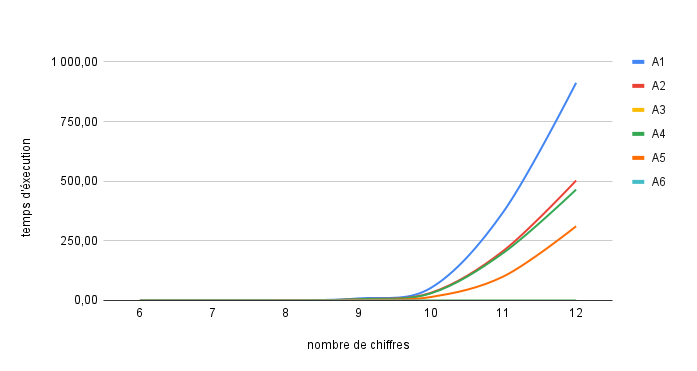
\includegraphics[scale=0.7]{chart1.png}
        \caption{Temps d'exécution des six algorithmes sur 7 nombres de chiffres différents }
    \label{fig:chart1}
\end{figure}
\\ \\

    
    \newpage
    \onehalfspacing
    \chapter{Mesure du temps d'exécution des 20 nombres premiers ayant la meme taille}
\section{Experimentation}
Le tableau suivant représente les temps d'exécution en nanoseconde de l'algorithme selon la variation des nombres premiers x1..x2 en ordre croissante.\\ \\
\par
\small
\resizebox{17cm}{!}{
\begin{tabular}{| c | c | c | c | c | c | c | c | c | c | c |}
    \hline
     x1 & x2 & x3 & x4 & x5 & x6 & x7 & x8 & x9 & x10   \\
    \hline
   1500450271 &
18790481837&
1979339339&
2030444287&
2860486313&
3267000013&
3367900313&
3628273133&
4093082899 & 4392489041\\
    \hline
    
     x11 & x12 & x13 & x14 & x15 & x16 & x17 & x18 & x19 & x20   \\
    \hline
    5038465463&
5463458053&
5555333227&
5754853343&
5915587277&
6668999101&
7896879971&
8278487999&
9471413089&
9576890767 \\
    \hline
\end{tabular}}
\\ \\
\par
\small
\resizebox{17cm}{!}{
\begin{tabular}{| c | c | c | c | c | c | c | c | c | c | c |}
    \hline
    x &  x1 & x2 & x3 & x4 & x5 & x6 & x7 & x8 & x9 & x10   \\
    \hline
    A1(s) & 16.113 &
20.109 &
19.987&
20.75&
44.815&
59.697&
48.246&
55.874&
68.331&
70.699
 \\
    \hline
    A2(s) & 8.206 &
9.687&
10.146&
15.69&
26.938&
28.324&
24.693&
31.044&
37.252&
34.662 \\
    \hline
    A3(s) &  0.002&
0.001&
0.001&
0.001&
0.001&
0.001&
0.001&
0.001&
0&
0.001\\
    \hline
    A4(s) & 8.198 &
10.035&
13.046&
17.019&
14.282&
20.343&
20.192&
22.26&
22.948&
25.089 \\
    \hline
    A5(s) & 4.429 &
5.178&
5.594&
5.062&
7.355&
8.195&
8.504&
9.544&
10.064&
11.134 \\
    \hline
    A6(s) & 0 &
0&
0&
0&
0.001&
0.001&
0.001&
0.001&
0.001&
0.001 \\
    \hline
\end{tabular}}
\\ \\
\par
\small
\resizebox{17cm}{!}{
\begin{tabular}{| c | c | c | c | c | c | c | c | c | c | c |}
    \hline
     &  x11 & x12 & x13 & x14 & x15 & x16 & x17 & x18 & x19 & x20   \\
    \hline
    A1(s) & 85.505&
59.221&
84.891&
68.61&
89.415&
94.345&
97.925&
93.204&
114.139&
152.4 \\
    \hline
    A2(s) & 28.492 &
48.4&
48.453&
50.096&
38.766&
34.916&
42.29&
48.979&
56.765&
106.045 \\
    \hline
    A3(s) & 0.002 &
0.001&
0.002&
0.001&
0.001&
0.002&
0.004&
0.004&
0.003&
0.002 \\
    \hline
    A4(s) & 29.859 &
34.864&
35.669&
34.387&
33.805&
36.295&
44.952&
44.042&
51.325&
52.909 \\
    \hline
    A5(s) & 12.632 &
13.641&
14.342&
14.516&
14.809&
20.352&
21.77&
21.964&
26.168&
24.905 \\
    \hline
    A6(s) &0.001&
0.001&
0&
0.001&
0.002&
0.001&
0.001&
0&
0.001&
0.001 \\
    \hline
\end{tabular}}
\\

\normalsize
\par
La figure suivante (voir Figure \ref{fig:chart}) représente l'évolution du temps d'exécution selon l'algorithme utilisee.

\begin{figure}[H]
    \centering
        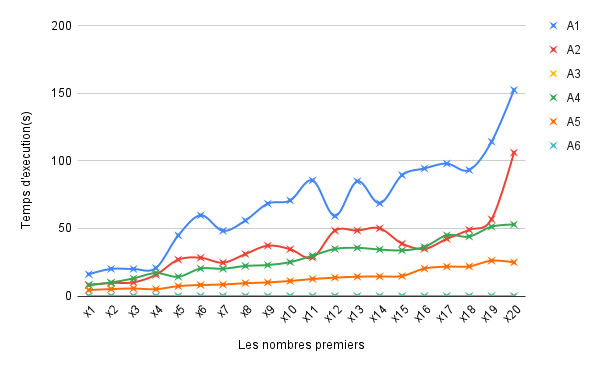
\includegraphics[scale=0.7]{chart.png}
        \caption{Temps d'exécution du programme selon l'algorithme utilisee}
    \label{fig:chart}
\end{figure}
\par
Depuis le graphe, les courbes  sont sous forme des arcs ascendants, on observe que le temps d’exécution évolue de manière presque linéarithmique avec l’augmentation des nombres premiers , avec A6 et A3 comme des meilleurs temps d'execution qui correspond bien à la complexité théorique calculée auparavant , On a pas obtenu une droite linéaire
car les testes étaient peu et aléatoires.

\section{Conclusion}
Les algorithmes A6 , A3 proposent une complexite optimale pour les tests de primalites quelque soit la taille de nombre. et pour ameliorer les resultats on veut tester les algorithmes plusieurs fois ce qu'on va voir dans le chapitre suivant .
    
    \newpage
    \onehalfspacing
    \chapter{Mesure du temps d'exécution apres 30 fois}
Le tableau suivant représente les temps d'exécution des six algorithmes  30 fois d'itérations sur des nombres ayant des longueurs différentes.
\\
\par
\small
\resizebox{17cm}{!}{
\begin{tabular}{| c | c | c | c | c | c | c | }
    \hline
    Nombre premier &  A1 & A2 & A3 & A4 & A5 & A6   \\
    \hline
 314159    &  0.003033 & 0.001400 & 0.000000  & 0.002200  & 0.000900   & 0.000033  
 \\
    \hline
4480649 &
0.040700 &
0.019367  &
0.000033   &
0.023600s &
0.005822  &
0.000033  \\
    \hline
    50943779 & 0.479900	& 0.231167 &	0.000200	& 0.332567 &	0.011132	& 0.000500  \\
    \hline
    999999937 & 8.502600	& 4.378000	& 0.000633	& 7.151200	& 2.185066 &	0.001267 \\
    \hline
    5915587277 & 49.763900 &	27.214133 &	0.001567 &	25.666167 &	12.863833 &	0.001767  \\
    \hline
    41996139943 & 795.541433 &	186.160400	& 0.003767	& 247.778366	& 92.497733 &	0.004233 \\
    \hline
    100123456789 & 957.670200 &	519.229133	& 0.006333 &	466.633330	& 268.685000 &	0.007533 \\
     \hline
\end{tabular}}
\\ \\
\normalsize
\par
La figure suivante (voir Figure \ref{fig:chart}) représente l'évolution du temps d'exécution selon l'algorithme utilisee.

\begin{figure}[H]
    \centering
        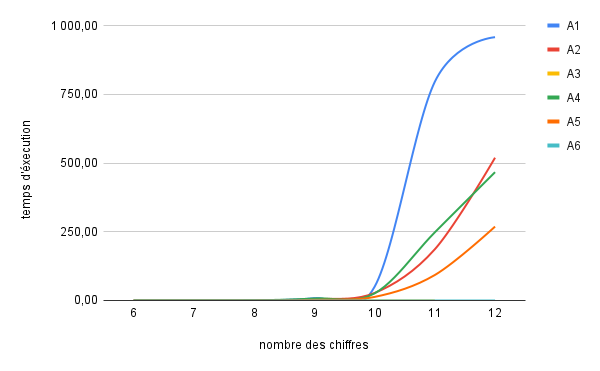
\includegraphics[scale=0.7]{chart2.png}
        \caption{Temps d'exécution des six algorithmes aprés 30 exécutions sur des nombres de longueurs différentes}
    \label{fig:chart}
\end{figure}
\\ 
A partir du graphe ci dessus, on constate qu'il y a une relation de correlation directe entre le nombre de chiffres et le temps d'éxecution moyen (plus que le nombre de chiffres auguemente plus que le temps d'éxecution auguemente)ce qui est le cas pour les algorithmes A1,A2,A4,A5.
\\
Pour le cas des algorithmes A3 et A6, on remarque que le résultat d'exécution tend vers 0 malgré l'augmentation du nombre de chiffres. 

    
    
    \newpage
    \onehalfspacing
    \chapter{Conclusion}
Beaucoup d'algorithmes existent, mais certains sont bien plus utilisés que d'autres en pratique. Le tri par insertion est souvent plébiscité pour des données de petite taille, tandis que des algorithmes asymptotiquement efficaces, comme le tri fusion, le tri par tas ou quicksort, seront utilisés pour des données de plus grande taille.
\\
La comparaison empirique d'algorithmes n'est pas aisée limitée au complexité de l'algorithme, il y'a beaucoup de paramètres entrent en compte : taille de données, ordre des données, matériel utilisé, taille de la mémoire vive, etc. 

    
    \newpage
    \onehalfspacing
    \chapter{Annexe :code source}
\section{Repartition des taches}
\par
\small
\resizebox{17cm}{!}{
\begin{tabular}{| c | c | }
    \hline
    Member &  Tache   \\
    \hline
    BEBNBACHIR Mohamed Amir & la conception de la solution iterative de hanoi + l'implementation en langage C + etude experimentale et analyse des resultats de la version iterative\\
    \hline
    BOUCHOUL Bouchra &  L'algorithme de verification avec calcule de sa complexite + Presentation d'une instance du probleme avec la solution (exemple)  \\
    \hline
    KHEMISSI Maroua &  Historique et presentation du probleme + Definition formelle du probleme+  Presentation de l'algorithme de resolution avec complexite theorique + representation de la modelisation de la solution\\
    \hline
    MEDJKOUNE Roumaissa & le programme de l'algorithme de résolution récursive en langage c + Son étude expérimentale + Analyse des résultats  \\
    \hline
  
\end{tabular}}
\\ \\
\newpage
\section{algorithme.c}
Le programme c 
\begin{minted}[
breaklines=true,
frame=lines,
linenos
]{c}
#include<stdio.h>
#include<stdlib.h>
#include<string.h>
#define MAX 100
#include<time.h>
//pile
struct discs {
	int size;
};
typedef discs *disc;
//les piles
typedef struct pile
{
    disc items[MAX];
    int top;
    int taille;
    int num;
} pile;

typedef struct Tour{
	int sizej;
	pile *A;
	pile *B;
	pile *C;
}Tour;
typedef Tour *TourH;


//les fonctions des piles
void initPile(pile *p,int num)
{
    p->top = -1;
    p->taille = 0;
    p->num=num;
}
int isempty(pile *p) {
   if (p->top == -1)
        return 1;
    else
        return 0;
}
int pilePleine(pile *s)
{
    if (s->top == MAX - 1)
        return 1;
    else
        return 0;
}
void push(pile *p, disc bt) {
 
    if (pilePleine(p))
    {
        printf("la pile est pleine");
    }
    else
    {
        p->top++;
        p->items[p->top] = bt;
    }
    p->taille++;

}
disc pop(pile *p) {
  if (isempty(p)){
  	return NULL;
  }
    p->taille--;
    disc val = p->items[p->top];
    p->top--;
    return val;
    }

///Initialiser le jeux en precisant le nombre initial des disques
TourH initHanoi(int size){
	TourH Tr= (TourH)malloc(sizeof(TourH));
	pile *A = (pile *)malloc(sizeof(pile));
    initPile(A,1);
    pile *B = (pile *)malloc(sizeof(pile));
    initPile(B,2);
    pile *C = (pile *)malloc(sizeof(pile));
    initPile(C,3);
    int i;
    for (i=size;i>0;i--){
    	disc d = (disc)malloc(sizeof(disc));
    	d->size=i;
    	push(A,d);
	}
    Tr->sizej=size;
    Tr->A=A;
    Tr->B=B;
    Tr->C=C;
 return Tr;
}

///fonction pou deplacer les disque entre les piles

void move(pile *p, pile *k,int* dep){
	disc d;
	d=pop(p);
	push(k,d);
	(*dep) += 1;
	
}

///fonctions tour d'hanoi
void Hanoi(int n,pile *A,pile *B,pile *C,int* dep){
	if (n>0){
	   Hanoi(n-1,A,C,B,dep);
	   move(A,C,dep);
	   Hanoi(n-1,B,A,C,dep);
	
	}
}

void moveI(pile * from ,pile * to){

    if (isempty(to))
    {
        push(to,pop(from));
    }
 
    else if (isempty(from))
    {
        push(from,pop(to));
    }
 
    else if (from->items[from->top]>to->items[to->top])
    {
        push(from,pop(to));
    }
 
    else
    {
        push(to,pop(from));
    }
}
void iterativeHanoi(int n,pile* start,pile* end,pile* inter){
    
    int total_num_of_moves = pow(2, n) - 1;
    
    
    if (n % 2 != 0)
    {
 
    for (int i = 1; i <= total_num_of_moves; i++)
    {
        if (i % 3 == 1)
        moveI(start,end);
 
        else if (i % 3 == 2)
        moveI(start,inter);
 
        else if (i % 3 == 0)
        moveI(inter,end);
    }
    }else{
        for (int i = 0; i < total_num_of_moves; i++)
    {
        if (i % 3 == 1)
        moveI(start,end);
 
        else if (i % 3 == 2)
        moveI(end,inter);
 
        else if (i % 3 == 0)
        moveI(inter,start);
    }
    }
}
void TourHanoi(TourH Tr,int* dep){
	Hanoi(Tr->sizej,Tr->A,Tr->B,Tr->C,dep);
}

int main(){
//enregistrement des executions

 clock_t t1,t2;
 double time;
 int j=5;
 FILE *f;
 f = fopen("nbDepHanoiRec.txt", "a");
  if (f != NULL)
    {  printf(" le fichier existe \n");}
    else
    { printf("Impossible d'ouvrir le fichier \n");}

 while(j<100){
     int d=0;
     TourH jeu= initHanoi(j);
     t1=clock();
     TourHanoi(jeu,&d);
     t2=clock();
     time=(float)(t2 - t1) / CLOCKS_PER_SEC;
     fprintf(f,"%d %d \n",j,d);
     j+=5;
 }


return 0;
}

\end{minted}
    
    \newpage
    \onehalfspacing
    \chapter{Références}
[1] Wikipedia .
\par
[2] Cours Algorithmique et Complexite - Prof DERIAS.H .



\end{document}
